% !TEX program = xelatex
% Biên dịch: xelatex slide_pcb.tex (chạy 2 lần); lualatex cũng dùng được.
% Đặt file ở thư mục gốc repo; ảnh lấy từ results/ và demo/assets/canary/.
% Quy ước: mỗi số liệu truy được về một file trong results/ hoặc configs/.
\PassOptionsToPackage{table}{xcolor}
\documentclass[aspectratio=169,11pt,t]{beamer}

%% ============================================================ THÔNG TIN (điền vào)
\newcommand{\presenter}{\texorpdfstring{%
  \begin{tabular}{@{}l@{\hspace{1.2em}}r@{}}
    \normalsize Đồng Nguyên Khôi & \normalsize MSV 24001677 \\
    \normalsize Phan Thanh Lâm & \normalsize MSV 24001680 \\
    \normalsize Nguyễn Vân Mạnh & \normalsize MSV 24001685
  \end{tabular}}{Nhóm 39}}
\newcommand{\course}{Giảng viên hướng dẫn: Hà Mạnh Toàn}
\newcommand{\when}{11/11/2026}

%% ============================================================ FONT
\usepackage{fontspec}
\IfFontExistsTF{Latin Modern Sans}{%
  \setsansfont{Latin Modern Sans}%
}{%
  \IfFontExistsTF{DejaVu Sans}{%
    \setsansfont{DejaVu Sans}%
  }{}%
}
\IfFontExistsTF{Latin Modern Mono}{%
  \setmonofont[Scale=0.95]{Latin Modern Mono}%
}{%
  \IfFontExistsTF{Liberation Mono}{%
    \setmonofont[Scale=0.92]{Liberation Mono}%
  }{%
    \setmonofont[Scale=0.9]{DejaVu Sans Mono}%
  }%
}
\renewcommand{\familydefault}{\sfdefault}
\usefonttheme{professionalfonts}

\usepackage{pifont}
\usepackage{xspace}
\usepackage{booktabs,array,tabularx}
\usepackage{tikz}
\usetikzlibrary{arrows.meta,positioning,calc,shapes.geometric,fit,backgrounds,decorations.pathreplacing}
\usepackage[most]{tcolorbox}
\usepackage{listings}
\graphicspath{{./}{../../}}

%% ============================================================ THEME
\usetheme{Madrid}

%% ============================================================ MÀU
\definecolor{ink}{HTML}{000000}
\definecolor{muted}{HTML}{666666}
\definecolor{hair}{HTML}{CCCCCC}
\definecolor{coral}{RGB}{51,51,178}
\definecolor{danger}{HTML}{C0392B}
\definecolor{teal}{HTML}{0E8A8C}
\definecolor{amber}{HTML}{D9930D}
\definecolor{indigo}{HTML}{8E44AD}
\definecolor{codebg}{HTML}{1B2333}
\definecolor{codefg}{HTML}{E6EAF2}
\definecolor{strc}{HTML}{8FE0B8}
\definecolor{cmt}{HTML}{8791A5}
\definecolor{kw}{HTML}{8FB8FF}
\definecolor{codeinl}{HTML}{B03A22}

%% Đồng bộ màu theme Madrid với màu chủ đạo
\setbeamercolor{structure}{fg=coral}
\setbeamercolor{palette primary}{bg=coral,fg=white}
\setbeamercolor{palette secondary}{bg=coral!85!black,fg=white}
\setbeamercolor{palette tertiary}{bg=coral!70!black,fg=white}
\setbeamercolor{title}{bg=coral,fg=white}
\setbeamertemplate{navigation symbols}{}
\setbeamertemplate{itemize items}[circle]
\hypersetup{pdftitle={Phát hiện và phân loại lỗi trên bảng mạch in (PCB): Báo cáo giữa kỳ},pdfauthor={Nhóm 39: Đồng Nguyên Khôi, Phan Thanh Lâm, Nguyễn Vân Mạnh}}

\setbeamersize{text margin left=1.2cm,text margin right=1.2cm}
\setbeamerfont{frametitle}{size=\large}
% \hl trong tiêu đề khung (chữ trắng trên nền xanh) chỉ in đậm, không đổi màu
\addtobeamertemplate{frametitle}{\let\hl\textbf}{\vskip-6pt}
\setbeamertemplate{bibliography item}[text]

% Bỏ dấu % ở dòng dưới để xem ghi chú nói cạnh slide (cần pgfpages, dùng 2 màn hình)
% \setbeameroption{show notes on second screen=right}

%% ============================================================ LỆNH & HỘP
\newcommand{\mycode}[1]{{\ttfamily\color{codeinl}#1}}
\newcommand{\hl}[1]{{\bfseries\color{coral}#1}}
\newcommand{\ok}{{\color{teal}\ding{51}}}
\newcommand{\no}{{\color{danger}\ding{55}}}
\newcommand{\num}[1]{\tikz[baseline=(c.base)]\node[circle,fill=coral,text=white,inner sep=0.6pt,minimum size=9pt,font=\bfseries\fontsize{6}{7}\selectfont](c){#1};}
\newcolumntype{L}[1]{>{\raggedright\arraybackslash\strut}p{#1}<{\strut}}
\newcommand{\cm}[1]{{\color{cmt}#1}}
\newcommand{\hdr}[1]{{\bfseries\color{muted}#1}}
\newcommand{\mynote}[1]{{\color{muted}\footnotesize #1}}

\setlength{\heavyrulewidth}{0.8pt}\setlength{\lightrulewidth}{0.4pt}
\arrayrulecolor{hair}

\tcbset{lbl/.style={enhanced,arc=2pt,frame hidden,left=8pt,right=7pt,top=4pt,bottom=4pt,
  boxsep=1pt,coltext=ink,nobeforeafter,halign=flush left}}
\newtcolorbox{why}[1][Giải thích]{lbl,borderline west={2.5pt}{0pt}{coral},colback=coral!9,
  before upper={\textbf{\textcolor{coral}{#1}}\enspace}}
\newtcolorbox{trap}[1][Lưu ý]{lbl,borderline west={2.5pt}{0pt}{amber},colback=amber!14,
  before upper={\textbf{\textcolor{amber!80!black}{#1}}\enspace}}
\newtcolorbox{key}[1][Kết luận]{lbl,borderline west={2.5pt}{0pt}{teal},colback=teal!9,
  before upper={\textbf{\textcolor{teal}{#1}}\enspace}}
\newtcolorbox{card}[2][]{enhanced,arc=3pt,colback=white,colframe=hair,boxrule=0.5pt,halign=flush left,
  borderline north={2pt}{0pt}{#2},left=7pt,right=7pt,top=5pt,bottom=5pt,#1}
% Khung nét đứt: phần chưa làm, để trống điền sau
\newtcolorbox{blank}[1][]{enhanced,arc=3pt,frame hidden,colback=white,halign=flush left,
  left=7pt,right=7pt,top=5pt,bottom=5pt,
  overlay={\draw[dashed,muted!70,line width=0.7pt,rounded corners=3pt]
    (frame.south west) rectangle (frame.north east);},#1}

%% ============================================================ CHÂN TRANG: lộ trình 5 phần
\newcommand{\navitem}[2]{\ifnum\insertsectionnumber=#1 {\bfseries\color{white}#2}\else{\color{white!58!coral}#2}\fi}
\setbeamertemplate{footline}{%
  \leavevmode\hbox{%
  \begin{beamercolorbox}[wd=.82\paperwidth,ht=2.6ex,dp=1.1ex,left,leftskip=1.2cm]{palette primary}%
    \fontsize{7}{8}\selectfont
    \navitem{1}{1 Bài toán}\quad\navitem{2}{2 Dữ liệu}\quad\navitem{3}{3 Phương pháp}\quad
    \navitem{4}{4 Kết quả}\quad\navitem{5}{5 Triển khai, kết luận}%
  \end{beamercolorbox}%
  \begin{beamercolorbox}[wd=.18\paperwidth,ht=2.6ex,dp=1.1ex,right,rightskip=1.0cm]{palette primary}%
    \fontsize{7}{8}\selectfont \insertframenumber/\inserttotalframenumber
  \end{beamercolorbox}}}

%% ============================================================ MÃ NGUỒN
\lstdefinestyle{dk}{
  basicstyle=\ttfamily\footnotesize\color{codefg},
  keywordstyle=\color{kw}\bfseries,stringstyle=\color{strc},commentstyle=\color{cmt},
  showstringspaces=false,escapeinside={(*@}{@*)},columns=fixed,keepspaces=true,
  upquote=false,breaklines=false,language={}}
\lstdefinestyle{dkx}{style=dk,basicstyle=\ttfamily\fontsize{8}{10}\selectfont\color{codefg}}
\newtcblisting{code}[1][]{listing only,enhanced,colback=codebg,colframe=codebg,boxrule=0pt,arc=3pt,
  left=7pt,right=5pt,top=5pt,bottom=5pt,before skip=2pt,after skip=4pt,
  listing options={style=dk,#1}}

\title[Phát hiện lỗi PCB]{Phát hiện và phân loại lỗi\\trên bảng mạch in (PCB)}
\subtitle{Báo cáo giữa kỳ, Nhóm 39}
\author[Nhóm 39]{\presenter}
\institute[GVHD: Hà Mạnh Toàn]{\course}
\date[\when]{\when}

\begin{document}

%% ============================================================ BÌA
\begin{frame}[c,plain]
  \titlepage
\end{frame}
\note{Giới thiệu nhóm và đề tài: phát hiện và phân loại lỗi trên bảng mạch in dựa trên hai hướng tiếp cận (đối chiếu ảnh mẫu và YOLO) cùng phương pháp kết hợp.}

%% ============================================================ NỘI DUNG
\begin{frame}{Nội dung trình bày}
  \centering
  \vspace{6pt}
  \begin{tikzpicture}[x=2.5cm, every node/.style={font=\sffamily}]
    \draw[coral!15, line width=5pt, line cap=round] (-0.45,0) -- (4.45,0);
    \foreach \i/\n/\t/\s in {
      0/1/{Bài toán}/{Đầu vào, đầu ra, độ đo đánh giá},
      1/2/{Dữ liệu}/{Bộ PKU Market PCB, chia theo bo},
      2/3/{Phương pháp}/{Đối chiếu ảnh mẫu, YOLO, phân loại, kết hợp},
      3/4/{Kết quả}/{Thực nghiệm, phân tích lỗi, so sánh},
      4/5/{Triển khai, kết luận}/{Demo, hạn chế, hướng phát triển}
    } {
      \node[circle, fill=coral, draw=white, line width=2pt, minimum size=1.05cm, inner sep=0pt, text=white, font=\bfseries\LARGE] (c\i) at (\i,0) {\n};
      \draw[coral!40, line width=1.2pt] (\i,-0.53) -- (\i,-0.75);
      \node[rounded corners=6pt, fill=coral!4, draw=coral!30, line width=0.8pt, text width=2.1cm, minimum height=1.7cm, align=center, inner sep=4pt, anchor=north] at (\i,-0.75) {%
        {\bfseries\small\color{coral!80!black}\t}\\[3pt]
        {\scriptsize\color{muted}\s}
      };
    }
  \end{tikzpicture}
\end{frame}

%% ============================================================ 1. BÀI TOÁN
\section{Bài toán}
\begin{frame}{Bài toán: phát hiện và phân loại lỗi trên \hl{bảng mạch in}}
  \footnotesize
  \textbf{Đầu vào:} ảnh bo mạch in $I$; với hướng đối chiếu, kèm ảnh mẫu không lỗi $T$ của cùng bo.\\[2pt]
  \textbf{Đầu ra:} tập dự đoán $\{(b_i,c_i,s_i)\}_{i=1}^{n}$, với $b_i=(x_1,y_1,x_2,y_2)$ là hộp bao, $c_i\in\{1,\dots,6\}$ là loại lỗi, $s_i\in[0,1]$ là độ tin cậy.
  \vspace{2pt}

  \centering
  \begin{tikzpicture}
    \foreach \f/\t [count=\i from 0] in {missing_hole/Missing Hole, mouse_bite/Mouse Bite, open_circuit/Open Circuit, short/Short, spur/Spur, spurious_copper/Spurious Copper} {
      \node[inner sep=0pt,draw=hair,line width=0.5pt] at ({\i*2.2},0) {\includegraphics[width=1.35cm]{../../demo/assets/canary/\f_1.png}};
      \node[font=\scriptsize,text=muted] at ({\i*2.2},-0.95) {\t};
    }
  \end{tikzpicture}
  \vspace{1pt}\par
  \mynote{Sáu lớp lỗi. Ảnh cắt 128$\times$128 quanh nhãn thật.}
  \vspace{1pt}

  \raggedright
  \begin{columns}[T,onlytextwidth]
    \begin{column}{0.48\textwidth}
      \begin{card}[height=2.6cm]{coral}
        \scriptsize \textbf{Đặc điểm của bài toán}
        \begin{itemize}\setlength{\itemsep}{0pt}
          \item Lỗi có kích thước nhỏ (vài chục pixel) so với ảnh toàn bo.
          \item Nền mạch lặp lại giữa các ảnh của cùng một bo.
          \item Một số chi tiết thiết kế có hình dạng tương tự lỗi.
        \end{itemize}
      \end{card}
    \end{column}
    \begin{column}{0.48\textwidth}
      \begin{card}[height=2.6cm]{teal}
        \scriptsize \textbf{Nội dung thực hiện}
        \begin{itemize}\setlength{\itemsep}{0pt}
          \item Cài đặt hai hướng: đối chiếu ảnh mẫu \cite{r1} và phát hiện trực tiếp bằng YOLOv8.
          \item Đề xuất kết hợp hai hướng để giảm dự đoán thừa.
          \item Đánh giá trên các bo không tham gia huấn luyện.
        \end{itemize}
      \end{card}
    \end{column}
  \end{columns}
\end{frame}
\note{Mô tả đầu vào, đầu ra và sáu lớp lỗi. Nhấn mạnh hai đặc điểm: lỗi nhỏ và nền lặp lại giữa các ảnh cùng bo. Nhóm sử dụng bộ PKU Market PCB gốc thay vì VOC\_PCB trong bản đăng ký, vì hướng đối chiếu cần ảnh nguyên bo và ảnh mẫu PCB\_USED.}

%% ============================================================ ĐỘ ĐO
\begin{frame}{Độ đo đánh giá}
  \begin{columns}[T]
    \begin{column}{0.54\textwidth}
      \footnotesize
      \textbf{Định vị và phát hiện (IoU $\ge$ 0,5)}
      \[ \mathrm{IoU}(b,g)=\frac{|b\cap g|}{|b\cup g|},\qquad F_1=\frac{2PR}{P+R} \]
      \[ P=\frac{TP}{TP+FP},\qquad R=\frac{TP}{TP+FN} \]
      Hộp dự đoán là $TP$ nếu có IoU $\ge 0{,}5$ với một nhãn cùng lớp chưa được ghép; nhầm lớp được tính là một $FP$ và một $FN$.\\[4pt]
      \textbf{Chất lượng mô hình phát hiện:} AP theo từng lớp, $\mathrm{mAP}_{50}$ và $\mathrm{mAP}_{50\text{--}95}$ (trung bình AP trên các ngưỡng IoU từ 0,5 đến 0,95).
    \end{column}
    \begin{column}{0.42\textwidth}
      \footnotesize
      \textbf{Sai số số lượng lỗi \cite{r1}}
      \[ P_d=\frac{|d-a|}{a}\times 100\% \]
      với $d$ là số vùng phát hiện, $a$ là số lỗi thật.\\[4pt]
      \textbf{Phân loại:} độ chính xác top-1 và ma trận nhầm lẫn.\\[4pt]
      \textbf{Phân tích lỗi:} mỗi dự đoán được xếp vào một trong bốn loại: \textit{đúng}, \textit{nhầm lớp}, \textit{bỏ sót}, \textit{thừa}.
    \end{column}
  \end{columns}
  \vspace{4pt}
  \begin{why}[Nhận xét:]
    \footnotesize $P_d$ chỉ so sánh số lượng, không kiểm tra vị trí; việc báo thừa và bỏ sót có thể bù trừ nhau. Vì vậy $P_d$ được báo cáo cùng $P$, $R$, $F_1$ theo IoU.
  \end{why}
\end{frame}
\note{Các độ đo được tính trên cùng tập test gồm 120 ảnh và 601 nhãn. $P_d$ giúp đối chiếu với công trình gốc; $P$, $R$, $F_1$ theo IoU kiểm tra thêm vị trí.}

%% ============================================================ 2. DỮ LIỆU
\section{Dữ liệu}
\begin{frame}{Bộ dữ liệu và phân chia theo \hl{ID bo}}
  \centering
  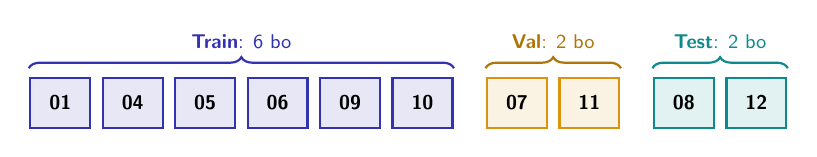
\begin{tikzpicture}[scale=0.8,transform shape]
    \foreach \b/\k [count=\i from 0] in {01/tr,04/tr,05/tr,06/tr,09/tr,10/tr,07/va,11/va,08/te,12/te} {
      \pgfmathsetmacro{\x}{\i*1.15+(\i>5?0.35:0)+(\i>7?0.35:0)}
      \ifnum\i<6 \def\cc{coral}\else\ifnum\i<8 \def\cc{amber}\else\def\cc{teal}\fi\fi
      \node[draw=\cc,fill=\cc!12,thick,minimum width=0.95cm,minimum height=0.8cm,font=\bfseries\small] at (\x,0) {\b};
    }
    \draw[decorate,decoration={brace,amplitude=4pt},coral,thick] (-0.5,0.55) -- (5*1.15+0.5,0.55)
      node[midway,above=5pt,font=\small,text=coral]{\textbf{Train}: 6 bo};
    \draw[decorate,decoration={brace,amplitude=4pt},amber!80!black,thick] ({6*1.15+0.35-0.5},0.55) -- ({7*1.15+0.35+0.5},0.55)
      node[midway,above=5pt,font=\small,text=amber!80!black]{\textbf{Val}: 2 bo};
    \draw[decorate,decoration={brace,amplitude=4pt},teal,thick] ({8*1.15+0.7-0.5},0.55) -- ({9*1.15+0.7+0.5},0.55)
      node[midway,above=5pt,font=\small,text=teal]{\textbf{Test}: 2 bo};
  \end{tikzpicture}
  \vspace{2pt}\par

  \begin{columns}[T,onlytextwidth]
    \begin{column}{0.52\textwidth}
      \footnotesize
      \renewcommand{\arraystretch}{1.25}\setlength{\tabcolsep}{4pt}
      \begin{tabular}{@{}L{1.0cm}L{3.4cm}rr@{}}
        \toprule
        \hdr{Tập} & \hdr{Bo} & \hdr{Ảnh} & \hdr{Hộp} \\
        \midrule
        Train & 01, 04, 05, 06, 09, 10 & 453 & 1749 \\
        Val & 07, 11 & 120 & 603 \\
        Test & 08, 12 & 120 & 601 \\
        \midrule
        \textbf{Tổng} & 10 bo & \textbf{693} & \textbf{2953} \\
        \bottomrule
      \end{tabular}
    \end{column}
    \begin{column}{0.44\textwidth}
      \begin{why}[Bộ PKU Market PCB \cite{r1}:]
        \scriptsize 693 ảnh lỗi của 10 bo, 6 lớp lỗi, 2953 hộp nhãn (định dạng Pascal VOC); lỗi được tạo bằng chỉnh sửa ảnh. Tên ảnh bắt đầu bằng ID bo.
      \end{why}
    \end{column}
  \end{columns}
  \vspace{3pt}
  \begin{key}[Nguyên tắc phân chia:]
    \scriptsize Mỗi bo thuộc đúng một tập, vì các ảnh cùng bo có nền mạch gần như giống nhau; phân chia ngẫu nhiên theo ảnh làm rò rỉ thông tin giữa huấn luyện và đánh giá. Các cách chia 6/2/2 được duyệt vét cạn với điều kiện mỗi tập đủ 6 lớp và số hộp trung bình mỗi bo giữa các tập chênh tối đa 1,03 lần. Kiểm tra rò rỉ: \mycode{results/data\_audit.csv}.
  \end{key}
\end{frame}
\note{Danh sách bo từng tập cố định trong \texttt{configs/board\_split.json}. Tổng 453 + 120 + 120 = 693 ảnh; 1749 + 603 + 601 = 2953 hộp.}

%% ============================================================ TIỀN XỬ LÝ
\begin{frame}{Tiền xử lý: chuyển nhãn \hl{VOC} sang \hl{YOLO} và cắt vùng lỗi}
  \centering
  \begin{tikzpicture}[
      bx/.style={rounded corners=4pt,fill=coral!6,draw=coral!40,thick,text width=2.75cm,minimum height=1.65cm,align=center,inner sep=4pt,font=\footnotesize},
      ar/.style={-{Stealth},thick,coral}]
    \node[bx] (a) at (0,0) {\textbf{Bộ PCB gốc}\\[2pt]\scriptsize \mycode{images/}, \mycode{Annotations/} (VOC), \mycode{PCB\_USED/}};
    \node[bx] (b) at (3.5,0) {\mycode{divide\_data.py}\\[2pt]\scriptsize kiểm tra XML, chia theo bo, đổi định dạng nhãn};
    \node[bx] (c) at (7.0,0) {\textbf{Dữ liệu YOLO theo bo}\\[2pt]\scriptsize \mycode{board\_split.json}, \mycode{data\_board.yaml}, \mycode{data\_audit.csv}};
    \node[bx] (d) at (10.5,0) {\mycode{collect\_crops.py}\\[2pt]\scriptsize ảnh cắt 128$\times$128 cho bộ phân loại};
    \draw[ar] (a) -- (b); \draw[ar] (b) -- (c); \draw[ar] (c) -- (d);
  \end{tikzpicture}
  \vspace{-3pt}\par

  \raggedright
  \begin{columns}[T,onlytextwidth]
    \begin{column}{0.52\textwidth}
      \begin{key}[Chuyển đổi nhãn:]
        \footnotesize Với ảnh kích thước $W\times H$ và hộp $(x_{\min},y_{\min},x_{\max},y_{\max})$ đã giới hạn trong khung ảnh:
        \[ x_c=\frac{x_{\min}+x_{\max}}{2W},\quad y_c=\frac{y_{\min}+y_{\max}}{2H} \]
        \[ w=\frac{x_{\max}-x_{\min}}{W},\quad h=\frac{y_{\max}-y_{\min}}{H} \]
        \scriptsize Chỉ số lớp theo thứ tự chữ cái: 0 Missing Hole, 1 Mouse Bite, 2 Open Circuit, 3 Short, 4 Spur, 5 Spurious Copper.
      \end{key}
    \end{column}
    \begin{column}{0.44\textwidth}
      \begin{why}[Ảnh cắt cho bộ phân loại:]
        \footnotesize Vùng vuông quanh hộp nhãn với lề 50\%, đưa về 128$\times$128, giữ nguyên cách chia theo bo: 1749 (train), 603 (val), 601 (test) ảnh cắt.
      \end{why}
    \end{column}
  \end{columns}
\end{frame}
\note{ID bo được tách từ phần tên ảnh trước dấu gạch dưới (ví dụ \texttt{08\_short\_01.jpg} thuộc bo 08).}

%% ============================================================ 3. PHƯƠNG PHÁP
\section{Phương pháp}
\begin{frame}{Tổng quan: hai hướng tiếp cận và \hl{phương pháp kết hợp}}
  \centering
  \begin{tikzpicture}[
      st/.style={rounded corners=4pt,fill=coral!6,draw=coral!40,thick,text width=2.35cm,minimum height=1.05cm,align=center,inner sep=3pt,font=\scriptsize},
      sy/.style={st,fill=teal!8,draw=teal!50},
      fu/.style={st,fill=amber!14,draw=amber!70,text width=3.6cm},
      ar/.style={-{Stealth},thick,coral!80}]
    \node[font=\scriptsize\bfseries,text=coral,anchor=west] at (-1.2,1.75) {Hướng đối chiếu ảnh mẫu \cite{r1}};
    \node[st] (a1) at (0,0.95) {Căn chỉnh: SIFT, lọc, RANSAC};
    \node[st] (a2) at (2.75,0.95) {Nhị phân hóa, XOR};
    \node[st] (a3) at (5.5,0.95) {Lọc nhiễu, lọc diện tích, tạo hộp};
    \node[st] (a4) at (8.25,0.95) {Phân loại vùng lỗi (YOLOv8n-cls)};
    \draw[ar] (a1)--(a2); \draw[ar] (a2)--(a3); \draw[ar] (a3)--(a4);

    \node[font=\scriptsize\bfseries,text=teal,anchor=west] at (-1.2,-0.55) {Hướng phát hiện trực tiếp};
    \node[sy] (b1) at (0,-1.35) {Ảnh lỗi, \mycode{imgsz}=1024};
    \node[sy] (b2) at (2.75,-1.35) {YOLOv8s};
    \node[sy] (b3) at (5.5,-1.35) {Hộp, lớp, độ tin cậy};
    \draw[ar,teal!80] (b1)--(b2); \draw[ar,teal!80] (b2)--(b3);

    \node[fu] (f) at (9.55,-0.2) {\textbf{Kết hợp}: giữ hộp YOLO nếu mặt nạ XOR xác nhận};
    \draw[ar,amber!80!black] (a4.south) to[bend left=15] (f.north);
    \draw[ar,amber!80!black] (b3.east) to[bend right=15] (f.south west);
  \end{tikzpicture}
  \vspace{2pt}\par

  \begin{columns}[T,onlytextwidth]
    \begin{column}{0.32\textwidth}
      \begin{card}[height=2.25cm]{coral}\footnotesize \textbf{Đối chiếu ảnh mẫu.} Yêu cầu ảnh không lỗi của đúng bo, cùng mặt và góc chụp gần giống; định vị chính xác chỗ khác biệt.\end{card}
    \end{column}
    \begin{column}{0.32\textwidth}
      \begin{card}[height=2.25cm]{teal}\footnotesize \textbf{YOLO.} Không yêu cầu ảnh mẫu, suy luận một giai đoạn; có thể nhầm chi tiết thiết kế của bo mới thành lỗi.\end{card}
    \end{column}
    \begin{column}{0.32\textwidth}
      \begin{card}[height=2.25cm]{amber}\footnotesize \textbf{Kết hợp.} Vị trí và nhãn lớp lấy từ YOLO; mặt nạ XOR đóng vai trò xác minh từng hộp.\end{card}
    \end{column}
  \end{columns}
\end{frame}
\note{Các file liên quan: \texttt{tools/baseline\_xor.py}, \texttt{pipeline.py}, \texttt{train.py}, \texttt{fusion.py}.}

%% ============================================================ ĐỐI CHIẾU ẢNH MẪU
\begin{frame}{Hướng đối chiếu ảnh mẫu: \hl{SIFT + XOR}}
  \begin{columns}[T]
    \begin{column}{0.56\textwidth}
      \small
      \num{1}\enspace \textbf{Ghép cặp:} ảnh lỗi $I$ với ảnh mẫu $T$ cùng ID bo.\\[3pt]
      \num{2}\enspace \textbf{Căn chỉnh:} trích đặc trưng SIFT, lọc tương ứng bằng tỉ lệ Lowe, ước lượng homography $H$ bằng RANSAC, biến đổi $I'=\mathrm{warp}(I,H)$.\\[3pt]
      \num{3}\enspace \textbf{Nhị phân hóa thích nghi} $I'$ và $T$ thành $B_I$, $B_T$; tính mặt nạ $M=B_I\oplus B_T$.\\[3pt]
      \num{4}\enspace \textbf{Lọc nhiễu:} loại vùng biên do warp; median blur, closing, opening và thành phần liên thông.\\[3pt]
      \num{5}\enspace \textbf{Tạo hộp:} lọc theo diện tích, mở rộng hộp quanh tâm, sau đó phân loại vùng lỗi.
    \end{column}
    \begin{column}{0.40\textwidth}
      \begin{why}[Căn chỉnh:]
        \footnotesize Điểm $x$ của $I$ được ánh xạ về khung của $T$ bởi homography $3\times3$: $x'\sim Hx$. RANSAC ước lượng $H$ bền vững với các cặp tương ứng sai.
      \end{why}
      \vspace{4pt}
      \begin{key}[Tham số (chọn trên val):]
        \footnotesize \mycode{close}=27, \mycode{min\_area}=250, \mycode{grow}=2,0.
      \end{key}
      \vspace{4pt}
      \begin{trap}[Thay đổi so với \cite{r1}:]
        \footnotesize SIFT thay SURF do SURF không có trong bản OpenCV miễn phí; bổ sung loại viền warp, nối mảnh XOR bằng closing lớn và mở rộng hộp.
      \end{trap}
    \end{column}
  \end{columns}
\end{frame}
\note{Hàm chính: \texttt{tools/baseline\_xor.py} (quy trình gốc) và \texttt{tools/pipeline.py} (bản cải tiến, dùng chung cho đánh giá và demo).}

%% ============================================================ YOLO
\begin{frame}{Hướng phát hiện trực tiếp: \hl{YOLOv8} và ngưỡng tin cậy theo lớp}
  \begin{columns}[T]
    \begin{column}{0.50\textwidth}
      \small
      \textbf{Mô hình:} YOLOv8n và YOLOv8s (Ultralytics \cite{r4}), khởi tạo từ trọng số tiền huấn luyện, phát hiện một giai đoạn trên ảnh nguyên bo.\\[4pt]
      \textbf{Cấu hình huấn luyện}
      \vspace{1pt}
      \footnotesize
      \renewcommand{\arraystretch}{1.2}\setlength{\tabcolsep}{4pt}
      \begin{tabular}{@{}L{3.0cm}L{3.2cm}@{}}
        \toprule
        Kích thước ảnh & 1024 (và 640) \\
        Batch / epoch tối đa & 8 / 100 \\
        Dừng sớm (patience) & 30 (dừng epoch 60, best 30) \\
        Seed & 0 \\
        Phần cứng & RTX 3050 6 GB \\
        \bottomrule
      \end{tabular}
    \end{column}
    \begin{column}{0.46\textwidth}
      \small
      \textbf{Ngưỡng tin cậy theo lớp.} Với mỗi lớp $c$, ngưỡng $\tau_c$ được chọn trên tập validation:
      \[
        \begin{aligned}
  \tau_c&=\arg\max_{\tau}\;F_1^{(c)}(\tau)\\
  &\text{với } R^{(c)}(\tau)\ge 0{,}90 .
\end{aligned}
      \]
      Kết quả: $\tau_{\text{Short}}=0{,}5$; các lớp còn lại $\tau_c=0{,}25$.\\[4pt]
      \begin{why}[Lựa chọn mô hình:]
        \footnotesize Mô hình được chọn trên validation theo $\mathrm{mAP}_{50\text{--}95}$ và số lỗi (bỏ sót, nhầm lớp). Tập test chỉ dùng để báo cáo.
      \end{why}
    \end{column}
  \end{columns}
\end{frame}
\note{Cấu hình ghi trong \texttt{configs/train\_params.md}. Mô hình chính dừng ở epoch 60, best epoch 30. Ngưỡng theo lớp: \texttt{configs/thresholds.json}.}

%% ============================================================ PHÂN LOẠI
\begin{frame}{Bộ phân loại vùng lỗi}
  \begin{columns}[T]
    \begin{column}{0.48\textwidth}
      \footnotesize
      \renewcommand{\arraystretch}{1.25}\setlength{\tabcolsep}{4pt}
      \begin{tabular}{@{}L{3.0cm}L{3.2cm}@{}}
        \toprule
        Mô hình & YOLOv8n-cls \\
        Đầu vào & ảnh cắt 128$\times$128, lề 50\% \\
        Số ảnh cắt & 1749 / 603 / 601 \\
        Batch / epoch tối đa & 64 / 50 \\
        Dừng sớm (patience) & 15 (epoch 31, best 16) \\
        \bottomrule
      \end{tabular}
    \end{column}
    \begin{column}{0.48\textwidth}
      \begin{why}[Vai trò:]
        \footnotesize Gán nhãn lớp cho các hộp do hướng đối chiếu ảnh mẫu tạo ra.
      \end{why}
      \vspace{4pt}
      \begin{key}[Hai chế độ đánh giá:]
        \footnotesize (i) trên ảnh cắt theo nhãn thật, cho cận trên của độ chính xác; (ii) trên hộp do bước XOR định vị đúng, phản ánh điều kiện sử dụng thực tế.
      \end{key}
    \end{column}
  \end{columns}
\end{frame}
\note{File: \texttt{tools/train\_cls.py}, \texttt{configs/train\_params.md}.}

\begin{frame}{Phương pháp kết hợp: \hl{YOLO + lọc bằng mặt nạ XOR}}
  \centering
  \begin{tikzpicture}[
      st/.style={rounded corners=4pt,fill=coral!6,draw=coral!40,thick,text width=3.0cm,minimum height=0.8cm,align=center,inner sep=3pt,font=\scriptsize},
      ar/.style={-{Stealth},thick,coral!80}]
    \node[st] (a) at (0,0) {Hộp YOLO (ngưỡng theo lớp)};
    \node[st,fill=amber!14,draw=amber!70,text width=4.3cm] (b) at (4.6,0) {Đếm pixel khác biệt của $M$ trong $b^{+\delta}$};
    \node[st,fill=teal!10,draw=teal!60,text width=2.4cm] (c) at (9.2,0.5) {$\ge \tau_{px}$: \textbf{giữ}};
    \node[st,fill=danger!8,draw=danger!60,text width=2.4cm] (d) at (9.2,-0.5) {$< \tau_{px}$: \textbf{loại}};
    \draw[ar] (a)--(b); \draw[ar] (b.east)--(c.west); \draw[ar] (b.east)--(d.west);
  \end{tikzpicture}
  \vspace{4pt}\par
  \raggedright
  \begin{key}[Quy tắc:]
    \footnotesize Gọi $b^{+\delta}$ là hộp $b$ mở rộng $\delta=8$ pixel và $M$ là mặt nạ XOR sau lọc nhiễu. Hộp được giữ khi
    \[ \sum_{p\in b^{+\delta}} M(p)\;\ge\;\tau_{px},\qquad \tau_{px}=10 . \]
    Hộp nằm gần viền đen do warp (không xác minh được) được giữ lại.
  \end{key}
  \vspace{3pt}
  \begin{why}[Cơ sở:]
    \footnotesize Chi tiết thiết kế cố định của bo trùng với ảnh mẫu nên không tạo pixel XOR; lỗi thật làm ảnh khác ảnh mẫu.
  \end{why}
  \vspace{3pt}
  \begin{trap}[Tính chất:]
    \footnotesize Phương pháp chỉ loại hộp, không thêm hộp, nên không làm tăng recall. $\tau_{px}$ được chọn trên validation với ràng buộc recall giảm không quá 0,01.
  \end{trap}
\end{frame}
\note{File: \texttt{tools/fusion.py}, \texttt{configs/fusion.json}.}

%% ============================================================ 4. KẾT QUẢ
\section{Kết quả}
\begin{frame}{Kết quả 1: so sánh các cấu hình \hl{YOLO} (validation)}
  \centering
  \scriptsize
  \renewcommand{\arraystretch}{1.3}\setlength{\tabcolsep}{4pt}
  \resizebox{\textwidth}{!}{%
  \begin{tabular}{@{}llrrrrrr@{}}
    \toprule
    \hdr{Cách chia} & \hdr{Mô hình, kích thước ảnh} & \hdr{P} & \hdr{R} & \hdr{mAP50} & \hdr{mAP50-95} & \hdr{ms/ảnh} \\
    \midrule
    Ngẫu nhiên & YOLOv8n, 1024 & 0,9702 & 0,9333 & 0,9668 & 0,5293 & 13,6 \\
    Ngẫu nhiên & YOLOv8s, 1024 & 0,9728 & 0,9473 & 0,9672 & 0,5437 & 24,9 \\
    Theo bo & YOLOv8n, 1024 & 0,9728 & 0,9165 & 0,9722 & 0,5195 & 13,3 \\
    \rowcolor{teal!12}
    \textbf{Theo bo} & \textbf{YOLOv8s, 1024} & \textbf{0,9752} & \textbf{0,9582} & \textbf{0,9782} & \textbf{0,5507} & \textbf{24,2} \\
    Theo bo & YOLOv8s, 640 & 0,9864 & 0,8945 & 0,9552 & 0,4963 & 11,7 \\
    \bottomrule
  \end{tabular}%
  }
  \vspace{5pt}\par

  \raggedright
  \begin{key}[Mô hình được chọn: YOLOv8s, chia theo bo, kích thước ảnh 1024.]
    \footnotesize $\mathrm{mAP}_{50\text{--}95}$ đạt 0,551 so với 0,519 của YOLOv8n; số hộp bỏ sót 11 so với 26; nhầm lớp 3 so với 11. Thời gian suy luận tăng từ 13,3 lên 24,2 ms/ảnh. Giảm kích thước ảnh xuống 640 làm recall giảm từ 0,958 xuống 0,895, phù hợp với đặc điểm lỗi kích thước nhỏ.
  \end{key}
  \vspace{2pt}
  \begin{trap}[Lưu ý:]
    \footnotesize Hai cách chia có tập validation khác nhau nên không so sánh trực tiếp. Validation gồm 2 bo và một seed; chênh lệch giữa các cấu hình mang tính chỉ thị.
  \end{trap}
\end{frame}
\note{Nguồn: \texttt{results/summary.csv}. Cấu hình pcb\_v8s (chia ngẫu nhiên) được chạy ngoài repo.}

\begin{frame}{Kết quả 2: YOLOv8s theo bo trên \hl{validation và test}}
  \begin{columns}[T]
    \begin{column}{0.52\textwidth}
      \footnotesize
      \renewcommand{\arraystretch}{1.35}\setlength{\tabcolsep}{2pt}
      \begin{tabular}{@{}lrrrr@{}}
        \toprule
        \hdr{Tập} & \hdr{P} & \hdr{R} & \hdr{mAP50} & \hdr{mAP50-95} \\
        \midrule
        Val (bo 07, 11) & 0,975 & 0,958 & 0,978 & 0,551 \\
        Test (bo 08, 12) & \cellcolor{danger!15}0,854 & 0,934 & 0,972 & 0,516 \\
        \bottomrule
      \end{tabular}
      \vspace{4pt}\par
      \mynote{Ngưỡng 0,25, kích thước ảnh 1024; 24,2 ms/ảnh (validation), 25,7 ms/ảnh (test). P, R là trung bình theo lớp (Ultralytics).}
    \end{column}
    \begin{column}{0.44\textwidth}
      \footnotesize
      \renewcommand{\arraystretch}{1.25}\setlength{\tabcolsep}{4pt}
      \begin{tabular}{@{}lrr@{}}
        \toprule
        \hdr{Lớp (test)} & \hdr{P} & \hdr{R} \\
        \midrule
        Missing Hole & \cellcolor{danger!15}0,627 & 0,980 \\
        Mouse Bite & 0,951 & 0,968 \\
        Open Circuit & 0,983 & 0,960 \\
        Short & \cellcolor{danger!15}0,613 & 0,990 \\
        Spur & 1,000 & \cellcolor{amber!25}0,714 \\
        Spurious Copper & 0,951 & 0,990 \\
        \bottomrule
      \end{tabular}
    \end{column}
  \end{columns}
  \vspace{4pt}
  \begin{key}[Nhận xét:]
    \small Từ validation sang test, $\mathrm{mAP}_{50}$ giảm 0,006 và recall giảm 0,024, trong khi precision giảm 0,121. Suy giảm precision tập trung ở hai lớp \textbf{Missing Hole} (0,627) và \textbf{Short} (0,613); lớp Spur có recall thấp nhất (0,714).
  \end{key}
\end{frame}
\note{Nguồn: \texttt{results/summary.csv}, \texttt{results/test\_metrics.csv}, \texttt{results/pcb\_v8s\_board\_test/metrics\_per\_class.csv}.}

\begin{frame}{Kết quả 3: phân tích lỗi, \hl{307 hộp thừa} trên test}
  \begin{columns}[T]
    \begin{column}{0.52\textwidth}
      \footnotesize
      \renewcommand{\arraystretch}{1.35}\setlength{\tabcolsep}{2.5pt}
      \begin{tabular}{@{}lrrrrr@{}}
        \toprule
        \hdr{Tập} & \hdr{Nhãn} & \hdr{Đúng} & \hdr{Nhầm lớp} & \hdr{Bỏ sót} & \hdr{Thừa} \\
        \midrule
        Validation & 603 & 589 & 3 & 11 & 20 \\
        Test & 601 & 573 & 6 & 22 & \cellcolor{danger!15}\textbf{307} \\
        \bottomrule
      \end{tabular}
      \vspace{4pt}\par
      \footnotesize \textbf{Vị trí hộp thừa:}\\[1pt]
      Validation: 18/20 lệch vị trí hoặc trùng với lỗi đã ghép.\\
      Test: \textbf{299/307} nằm trên vùng nền (IoU dưới 0,1 với mọi nhãn).
    \end{column}
    \begin{column}{0.44\textwidth}
      \centering
      \begin{tikzpicture}[x=0.022cm,y=1cm]
        \node[font=\scriptsize\bfseries,text=muted,anchor=south] at (62,0.35) {Hộp thừa theo lớp (test)};
        \foreach \n/\v/\c [count=\i] in {Short/123/danger, Missing Hole/119/danger, Spurious Copper/55/coral, Mouse Bite/7/coral, Spur/2/coral, Open Circuit/1/coral} {
          \node[anchor=east,font=\scriptsize] at (-4,{-\i*0.52+0.3}) {\n};
          \fill[\c!75] (0,{-\i*0.52+0.3-0.17}) rectangle (\v,{-\i*0.52+0.3+0.17});
          \node[anchor=west,font=\scriptsize] at ({\v+3},{-\i*0.52+0.3}) {\v};
        }
      \end{tikzpicture}
    \end{column}
  \end{columns}
  \vspace{3pt}
  \begin{why}[Giải thích sự khác biệt giữa mAP và precision:]
    \footnotesize Các hộp thừa có độ tin cậy thấp đến trung bình (trung bình theo lớp 0,31 đến 0,56). AP là tích phân trên toàn bộ đường precision--recall nên ít chịu ảnh hưởng ($\mathrm{mAP}_{50}$: 0,978 $\to$ 0,972), còn precision được đo tại một ngưỡng cố định (0,975 $\to$ 0,854).
  \end{why}
\end{frame}
\note{Nguồn: \texttt{results/pcb\_v8s\_board\_*\_errors/}, \texttt{reports/bang\_so\_lieu.md}. Phân tích bằng \texttt{tools/analyze\_errors.py}, ghép hộp dự đoán với nhãn ở IoU 0,5.}

\begin{frame}{Kết quả 4: hộp thừa tập trung tại \hl{vị trí cố định}}
  \footnotesize
  \renewcommand{\arraystretch}{1.3}\setlength{\tabcolsep}{4pt}
  \begin{tabular}{@{}L{1.0cm}L{3.2cm}L{2.8cm}rrL{3.0cm}@{}}
    \toprule
    \hdr{Bo} & \hdr{Lớp bị báo} & \hdr{Vị trí (x, y)} & \hdr{Ảnh} & \hdr{conf} & \hdr{Sau ngưỡng theo lớp} \\
    \midrule
    08 & Missing Hole & 180, 1080 & 60 & 0,59 & còn \\
    08 & Missing Hole & 1740, 510 & 59 & 0,34 & còn \\
    12 & Short & 1170, 1140 & 60 & 0,63 & còn \\
    12 & Short & 1560, 1110 & 60 & 0,39 & \cellcolor{teal!15}bị loại \\
    12 & Spurious Copper & 1710, 1560 & 51 & 0,32 & còn \\
    \bottomrule
  \end{tabular}
  \vspace{2pt}\par
  \mynote{Ảnh: số ảnh (trên 60 ảnh của bo) có hộp thừa tại vị trí đó. conf: độ tin cậy trung bình. Vị trí gom theo tâm hộp, làm tròn 30 px.}
  \vspace{4pt}
  \begin{key}[Kết quả:]
    \small \textbf{290/307 (94,5\%)} hộp thừa nằm ở đúng 5 vị trí; mỗi vị trí xuất hiện ở 51 đến 60 trong 60 ảnh của cùng một bo. 17 hộp còn lại phân tán.
  \end{key}
  \vspace{1pt}
  \begin{why}[Diễn giải:]
    \small Nếu là sai số ngẫu nhiên thì vị trí hộp thừa sẽ thay đổi giữa các ảnh. Sự lặp lại tại cùng một vị trí trên hầu hết ảnh của một bo cho thấy mô hình phản ứng với \textbf{một chi tiết cố định của bo đó}.
  \end{why}
\end{frame}
\note{Nguồn: \texttt{reports/bang\_so\_lieu.md}, mục 5.}

\begin{frame}{Kết quả 4 (tiếp): các vị trí đó là \hl{chi tiết của bo}}
  \centering
  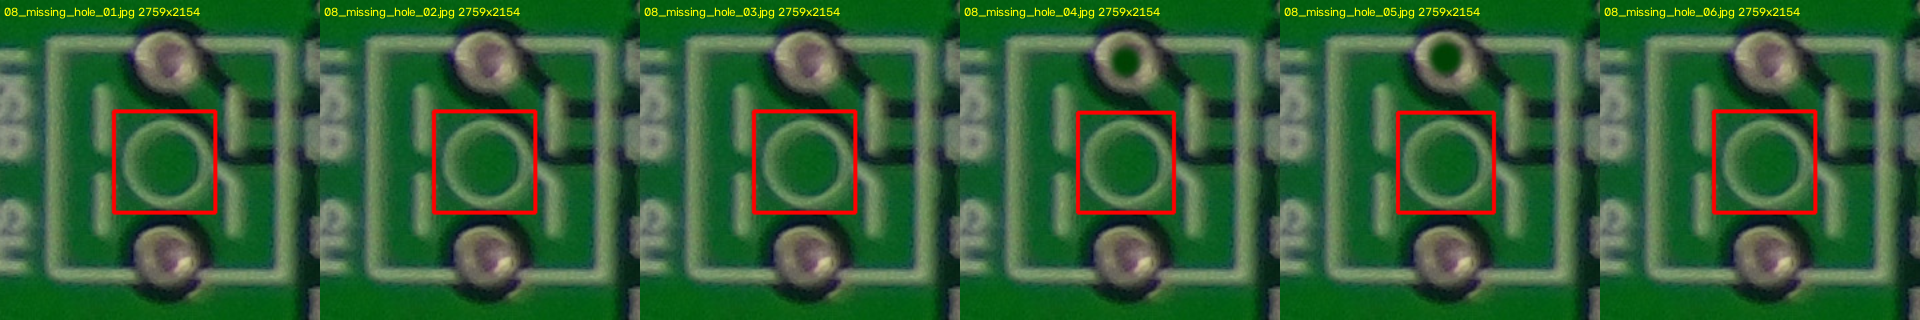
\includegraphics[width=0.58\textwidth]{../../results/hotspot2_08_180_1080.png}\par
  \mynote{Bo 08, vị trí (180, 1080), 6 ảnh test khác nhau (ảnh lớp Missing Hole). Hộp đỏ là vị trí hộp thừa.}
  \vspace{2pt}\par
  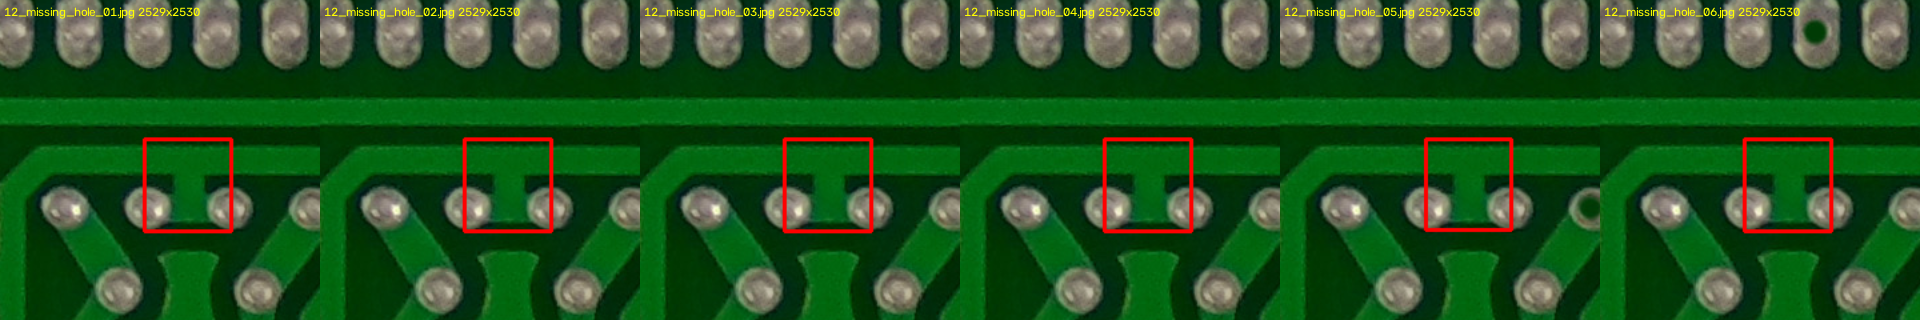
\includegraphics[width=0.58\textwidth]{../../results/hotspot2_12_1170_1140.png}\par
  \mynote{Bo 12, vị trí (1170, 1140), 6 ảnh test khác nhau.}
  \vspace{1pt}
  \raggedright\scriptsize
  \begin{itemize}
    \item Bo 08, hộp \mycode{145, 1043, 221, 1119} giống nhau đến từng pixel trong 54/60 ảnh và xuất hiện ở 10 ảnh của \textbf{mỗi} lớp lỗi; nhãn lỗi bị thiếu không thể xuất hiện ở ảnh của mọi lớp.
    \item Mô hình nhầm các cấu trúc trông giống lỗi: vòng tròn rỗng giống lỗ thiếu, chỗ nối hoặc giao đường mạch giống đoản mạch, đoạn đồng lẻ giống đồng thừa.
  \end{itemize}
  \begin{trap}[Hạn chế:]
    \scriptsize Điểm (1170, 1140) của bo 12 có thể là thiết kế hợp lệ hoặc lỗi có sẵn trên bo gốc nhưng không được gán nhãn; chưa phân biệt được từ ảnh.
  \end{trap}
\end{frame}
\note{Ảnh: \texttt{results/hotspot2\_*.png}, sinh bằng \texttt{tools/crop\_hotspot\_v2.py}.}

\begin{frame}{Kết quả 5: khảo sát ngưỡng và \hl{ngưỡng theo lớp}}
  \begin{columns}[T]
    \begin{column}{0.50\textwidth}
      \footnotesize
      \renewcommand{\arraystretch}{1.3}\setlength{\tabcolsep}{4pt}
      \renewcommand{\arraystretch}{1.1}\renewcommand{\arraystretch}{1.1}\resizebox{0.95\textwidth}{!}{%
      \begin{tabular}{@{}rrrrrr@{}}
        \toprule
        \hdr{conf} & \hdr{P} & \hdr{R} & \hdr{F1} & \hdr{Sai} & \hdr{Sót} \\
        \midrule
        \rowcolor{teal!12}0,25 & 0,962 & 0,977 & 0,970 & 23 & 11 \\
        0,40 & 0,976 & 0,954 & 0,965 & 14 & 25 \\
        0,50 & 0,981 & 0,942 & 0,961 & 11 & 33 \\
        0,60 & 0,987 & 0,905 & 0,945 & 7 & 56 \\
        \bottomrule
      \end{tabular}%
      }
      \vspace{2pt}\par
      \mynote{Validation; P, R gộp trên tất cả hộp. \textit{Sai}: hộp thừa và nhầm lớp; \textit{Sót}: nhãn không được phát hiện.}
    \end{column}
    \begin{column}{0.46\textwidth}
      \footnotesize
      \begin{card}[height=2.2cm]{coral}
        \textbf{Ngưỡng theo lớp} (Short 0,5; các lớp còn lại 0,25):\\[3pt]
        trên test, số hộp đúng (573) và bỏ sót (22) giữ nguyên; hộp thừa giảm \textbf{307 $\to$ 245}.
      \end{card}
    \end{column}
  \end{columns}
  \vspace{2pt}
  \begin{key}[Nhận xét:]
    \scriptsize Tăng ngưỡng chung từ 0,25 lên 0,40 chỉ giảm 9 hộp sai (23 $\to$ 14) nhưng tăng 14 hộp bỏ sót (11 $\to$ 25); đường F1 gần phẳng trong khoảng 0,2 đến 0,6.
  \end{key}
  \vspace{2pt}
  \begin{trap}[Hạn chế của ngưỡng:]
    \footnotesize Mức giảm 62 hộp tương ứng với vị trí Short tại (1560, 1110). Trong 245 hộp thừa còn lại, 229 hộp nằm ở 4 vị trí còn lại, trong đó hai điểm có độ tin cậy trung bình 0,59 và 0,63 nên không thể loại bằng ngưỡng mà không mất hộp đúng.
  \end{trap}
\end{frame}
\note{Nguồn: \texttt{configs/thresholds.json}, \texttt{reports/bang\_so\_lieu.md}.}

\begin{frame}{Kết quả 6: hướng đối chiếu ảnh mẫu, \hl{định vị}}
  \begin{columns}[T]
    \begin{column}{0.46\textwidth}
      \footnotesize
      \renewcommand{\arraystretch}{1.3}\setlength{\tabcolsep}{3pt}
      \begin{tabular}{@{}lrrrrrr@{}}
        \toprule
        & \multicolumn{3}{c}{\hdr{Validation}} & \multicolumn{3}{c}{\hdr{Test}} \\
        \cmidrule(lr){2-4}\cmidrule(l){5-7}
        \hdr{IoU} & \hdr{P} & \hdr{R} & \hdr{F1} & \hdr{P} & \hdr{R} & \hdr{F1} \\
        \midrule
        0,5 & 0,620 & 0,615 & 0,618 & 0,656 & 0,621 & 0,638 \\
        0,3 & 0,955 & 0,947 & 0,951 & 0,972 & 0,920 & 0,945 \\
        0,1 & 0,997 & 0,988 & 0,993 & 0,981 & 0,929 & 0,954 \\
        \bottomrule
      \end{tabular}
      \vspace{3pt}\par
      \mynote{Số hộp dự đoán: validation 598 (nhãn 603), test 569 (nhãn 601). Chỉ xét định vị, chưa tính lớp.}
    \end{column}
    \begin{column}{0.50\textwidth}
      \footnotesize
      \begin{key}[Nhận xét:]
        Ở IoU 0,5, $F_1$ trên test đạt 0,638; ở IoU 0,3 đạt 0,945 (số hộp khớp tăng từ 373 lên 553 trên 601 nhãn). Vùng khác biệt được định vị đúng nhưng nhiều hộp chưa khớp đủ chặt với nhãn về kích thước.
      \end{key}
      \vspace{4pt}
      \begin{why}[Sai số số lượng:]
        $P_d=|569-601|/601=5{,}32\%$ trên test; $0{,}83\%$ trên validation.
      \end{why}
    \end{column}
  \end{columns}
\end{frame}
\note{Nguồn: \texttt{results/pipeline\_val.csv}, \texttt{pipeline\_test.csv} (biến thể cải tiến). Việc ghép hộp theo IoU không xét lớp; phân loại được đo ở slide kế tiếp.}

\begin{frame}{Kết quả 7: phân loại vùng lỗi, nhầm lẫn giữa \hl{Spur} và \hl{Spurious Copper}}
  \begin{columns}[T]
    \begin{column}{0.46\textwidth}
      \footnotesize
      \begin{itemize}
        \item Trên \textbf{hộp nhãn thật}: top-1 validation 1,000; test 0,990 (595/601), là cận trên vì không tính sai số định vị. Sai 6 ảnh: 5 Spur thành Spurious Copper, 1 Mouse Bite thành Open Circuit.
        \item Trên \textbf{hộp XOR định vị đúng}: 342/373 = 0,917.
      \end{itemize}
    \end{column}
    \begin{column}{0.50\textwidth}
      \centering
      \footnotesize
      \renewcommand{\arraystretch}{1.25}\setlength{\tabcolsep}{5pt}
      \begin{tabular}{@{}l rrrrrr@{}}
        & \multicolumn{6}{c}{\hdr{Dự đoán}} \\
        \hdr{Thật} & \hdr{MH} & \hdr{MB} & \hdr{OC} & \hdr{Sh} & \hdr{Sp} & \hdr{SC} \\
        \midrule
        MH & \cellcolor{teal!18}33 & {\color{hair}0} & {\color{hair}0} & {\color{hair}0} & {\color{hair}0} & {\color{hair}0} \\
        MB & {\color{hair}0} & \cellcolor{teal!18}86 & \cellcolor{danger!22}1 & {\color{hair}0} & {\color{hair}0} & {\color{hair}0} \\
        OC & {\color{hair}0} & {\color{hair}0} & \cellcolor{teal!18}86 & {\color{hair}0} & {\color{hair}0} & {\color{hair}0} \\
        Sh & {\color{hair}0} & {\color{hair}0} & {\color{hair}0} & \cellcolor{teal!18}62 & {\color{hair}0} & \cellcolor{danger!22}2 \\
        Sp & {\color{hair}0} & {\color{hair}0} & {\color{hair}0} & {\color{hair}0} & \cellcolor{amber!30}19 & \cellcolor{danger!40}28 \\
        SC & {\color{hair}0} & {\color{hair}0} & {\color{hair}0} & {\color{hair}0} & {\color{hair}0} & \cellcolor{teal!18}56 \\
      \end{tabular}
      \vspace{2pt}\par
      \mynote{Test, hộp XOR định vị đúng (n = 373). MH Missing Hole, MB Mouse Bite, OC Open Circuit, Sh Short, Sp Spur, SC Spurious Copper.}
    \end{column}
  \end{columns}
  \vspace{3pt}
  \begin{key}[Nhận xét:]
    \small Spur chỉ đạt 19/47 = 0,40 (28 hộp bị gán thành Spurious Copper); năm lớp còn lại đạt từ 0,969 đến 1,000. Giả thuyết: hai lớp đều là phần đồng nhỏ nhô ra cạnh đường mạch nên ảnh cắt 128$\times$128 có hình thái gần giống nhau.
  \end{key}
\end{frame}
\note{Nguồn: \texttt{results/pipeline\_test\_cls.csv}; top-1 trên ảnh cắt: \texttt{configs/train\_params.md}. Do đó nhãn lớp trong phương pháp kết hợp được lấy từ YOLO.}

\begin{frame}{Kết quả 8: \hl{YOLO + lọc XOR} trên test}
  \centering
  \footnotesize
  \renewcommand{\arraystretch}{1.3}\setlength{\tabcolsep}{6pt}
  \begin{tabular}{@{}lrrrrrr@{}}
    \toprule
    \hdr{Test, IoU 0,5} & \hdr{TP} & \hdr{FP} & \hdr{FN} & \hdr{P} & \hdr{R} & \hdr{F1} \\
    \midrule
    YOLOv8s thuần & 573 & 368 & 28 & 0,609 & 0,953 & 0,743 \\
    \rowcolor{teal!12}
    \textbf{YOLOv8s + lọc XOR} & \textbf{573} & \textbf{20} & \textbf{28} & \textbf{0,966} & \textbf{0,953} & \textbf{0,960} \\
    \bottomrule
  \end{tabular}
  \vspace{6pt}\par
  \begin{columns}[T,onlytextwidth]
    \begin{column}{0.52\textwidth}
      \footnotesize
      \renewcommand{\arraystretch}{1.25}\setlength{\tabcolsep}{2pt}
      \begin{tabular}{@{}lrrr@{}}
        \toprule
        \hdr{Lớp (test)} & \hdr{FP thuần} & \hdr{FP + XOR} & \hdr{P + XOR} \\
        \midrule
        Missing Hole & 238 & \cellcolor{teal!15}0 & 1,000 \\
        Mouse Bite & 8 & 8 & 0,923 \\
        Open Circuit & 1 & 1 & 0,990 \\
        Short & 61 & \cellcolor{teal!15}2 & 0,980 \\
        Spur & 1 & 1 & 0,988 \\
        Spurious Copper & 59 & \cellcolor{teal!15}8 & 0,925 \\
        \bottomrule
      \end{tabular}
    \end{column}
    \begin{column}{0.44\textwidth}
      \raggedright
      \begin{key}[Nhận xét:]
        \footnotesize Phương pháp loại 348/368 hộp thừa mà không làm mất hộp đúng nào (TP giữ nguyên 573): $P$ tăng 0,609 $\to$ 0,966, $F_1$ tăng 0,743 $\to$ 0,960. Hiệu quả tập trung ở ba lớp có vị trí lặp lại.
      \end{key}
    \end{column}
  \end{columns}
\end{frame}
\note{Nguồn: \texttt{results/fusion\_test.csv}. $P$, $R$ ở đây là chỉ số gộp, khớp cùng lớp ở IoU 0,5, nên số FP (368) khác số hộp thừa (307, 245) ở các slide trước do cách ghép khác nhau. Test được chạy một lần, 0 ảnh căn chỉnh thất bại.}

\begin{frame}{Kết quả 8 (tiếp): độ nhạy của tham số \hl{$\tau_{px}$}}
  \begin{columns}[T]
    \begin{column}{0.46\textwidth}
      \footnotesize
      \renewcommand{\arraystretch}{1.3}\setlength{\tabcolsep}{5pt}
      \begin{tabular}{@{}rrrr@{}}
        \toprule
        \hdr{$\tau_{px}$} & \hdr{FP} & \hdr{FN} & \hdr{F1} \\
        \midrule
        0 & 18 & 15 & 0,9727 \\
        \rowcolor{teal!12}10 & 17 & 15 & 0,9735 \\
        100 & 17 & 15 & 0,9735 \\
        200 & 17 & 19 & 0,9701 \\
        400 & 15 & 48 & 0,9463 \\
        800 & 12 & 310 & 0,6454 \\
        \bottomrule
      \end{tabular}
      \vspace{2pt}\par
      \mynote{Khảo sát $\tau_{px}$ trên validation.}
    \end{column}
    \begin{column}{0.50\textwidth}
      \begin{key}[Nhận xét:]
        \footnotesize $F_1$ trên validation ổn định với $\tau_{px}$ từ 10 đến 100 và giảm từ 200 khi recall bắt đầu suy giảm; giá trị 10 được chọn.
      \end{key}
      \vspace{4pt}
      \begin{trap}[Hạn chế:]
        \footnotesize Tập validation gần như không có vị trí lặp lại (18 $\to$ 17 hộp thừa) nên việc chọn $\tau_{px}$ trên validation chủ yếu kiểm tra ràng buộc recall; hiệu quả loại hộp thừa thể hiện chủ yếu trên test.
      \end{trap}
    \end{column}
  \end{columns}
\end{frame}
\note{Nguồn: \texttt{results/fusion\_val\_sweep.csv}.}

\begin{frame}{So sánh với công trình gốc \cite{r1}: sai số số lượng \hl{$P_d$}}
  \footnotesize
  \renewcommand{\arraystretch}{1.3}\setlength{\tabcolsep}{5pt}
  \begin{tabular}{@{}L{4.4cm}L{3.5cm}rrr@{}}
    \toprule
    \hdr{Phương pháp} & \hdr{Tập đánh giá} & \hdr{$d$} & \hdr{$a$} & \hdr{$P_d$} \\
    \midrule
    Công trình gốc \cite{r1} (SURF + XOR) & Toàn bộ 693 ảnh & 2955 & 2953 & 0,07\% \\
    XOR cải tiến (nhóm) & Validation & 598 & 603 & 0,83\% \\
    XOR cải tiến (nhóm) & Test & 569 & 601 & 5,32\% \\
    YOLOv8s thuần & Test & 941 & 601 & 56,57\% \\
    \rowcolor{teal!12}
    \textbf{YOLOv8s + lọc XOR} & Test & \textbf{593} & \textbf{601} & \textbf{1,33\%} \\
    \bottomrule
  \end{tabular}
  \vspace{6pt}\par
  \begin{trap}[Lưu ý khi so sánh:]
    \footnotesize Công trình gốc đánh giá trên toàn bộ 693 ảnh, không có tập giữ lại, và không báo cáo $P$, $R$ theo IoU hay mAP. Nhóm đánh giá trên 2 bo không dùng khi chọn tham số. $P_d$ chỉ so sánh số lượng nên cần đặt cạnh $P$, $R$ theo IoU: $F_1$ của XOR cải tiến là 0,638, của YOLOv8s + lọc XOR là 0,960.
  \end{trap}
\end{frame}
\note{Công thức $P_d$ theo công trình gốc. YOLO thuần có 941 dự đoán nên $P_d$ = 56,57\% do hộp thừa. $P_d$ thấp không bảo đảm đúng vị trí.}

\begin{frame}{So sánh với công trình gốc \cite{r1}: phân loại và \hl{thời gian}}
  \footnotesize
  \renewcommand{\arraystretch}{1.3}\setlength{\tabcolsep}{5pt}
  \begin{tabular}{@{}L{4.4cm}L{3.9cm}L{3.9cm}@{}}
    \toprule
    \hdr{Chỉ số} & \hdr{Công trình gốc \cite{r1}} & \hdr{Nhóm} \\
    \midrule
    Phân loại trên ảnh cắt theo nhãn (test) & 97,74\% & 0,990 (top-1) \\
    Phân loại trên vùng do bước định vị tìm ra & 99,40\% & 0,917 \\
    Thời gian một ảnh & 0,9889 s (đăng ký ảnh 0,6219 s) & YOLO 25,71 ms; đường XOR: chưa đo \\
    \bottomrule
  \end{tabular}
  \vspace{6pt}\par
  \begin{key}[Nhận xét:]
    \footnotesize Trên ảnh cắt theo nhãn, độ chính xác của nhóm cao hơn. Trên vùng do bước định vị tìm ra, kết quả thấp hơn công trình gốc, tập trung ở lớp Spur (0,40); các lớp còn lại đạt 0,969 đến 1,000.
  \end{key}
  \vspace{3pt}
  \begin{trap}[Lưu ý khi so sánh:]
    \scriptsize Thiết lập khác nhau (kích thước ảnh cắt, cách chia dữ liệu, bộ phân loại, phần cứng); công trình gốc không nêu rõ có chia theo bo hay không. Thời gian của YOLO đo trên RTX 3050, không gồm đăng ký ảnh, nên không so sánh trực tiếp. Giả thuyết cho chênh lệch ở vùng tìm ra (bộ phân loại nhận ảnh cắt từ hộp XOR, phóng hệ số 2,0) chưa được kiểm chứng.
  \end{trap}
\end{frame}
\note{Công trình gốc nhận xét ảnh cắt từ so sánh với ảnh mẫu nhỏ hơn ảnh cắt theo nhãn. Kết quả ngược chiều của hai nghiên cứu chưa được giải thích đầy đủ.}

%% ============================================================ 5. TRIỂN KHAI, KẾT LUẬN
\section{Triển khai, kết luận}
\begin{frame}{Hệ thống demo}
  \begin{columns}[T]
    \begin{column}{0.58\textwidth}
      \footnotesize
      \renewcommand{\arraystretch}{1.25}\setlength{\tabcolsep}{2pt}
      \begin{tabular}{@{}L{2.2cm}L{2.4cm}L{3.0cm}@{}}
        \toprule
        \hdr{Chức năng} & \hdr{Đầu vào} & \hdr{Phương pháp} \\
        \midrule
        Phát hiện nhanh & một ảnh & YOLOv8s \\
        Đối chiếu ảnh mẫu & ảnh + ảnh bo chuẩn & SIFT, XOR, phân loại \\
        Đối chiếu hai hướng & ảnh + ảnh bo chuẩn & cả hai, ghép hộp ở IoU $\geq$ 0,1 \\
        \bottomrule
      \end{tabular}
      \vspace{6pt}\par
      \begin{why}[Cơ chế an toàn:]
        \scriptsize Kiểm tra đầu vào (loại, kích thước, giải mã); tự kiểm tra bộ phân loại bằng 12 ảnh mẫu khi khởi động; chuyển sang CPU khi hết bộ nhớ GPU; thông báo khi căn chỉnh thất bại.
      \end{why}
    \end{column}
    \begin{column}{0.38\textwidth}
      \begin{card}[height=3.6cm]{amber}
        \footnotesize \textbf{Chức năng đối chiếu hai hướng}\\[4pt]
        \tikz[baseline=-0.5ex]\draw[fill=teal!25,draw=teal,thick](0,-0.12) rectangle (0.5,0.12);\enspace Cả hai hướng cùng phát hiện\\[4pt]
        \tikz[baseline=-0.5ex]\draw[fill=coral!25,draw=coral,thick](0,-0.12) rectangle (0.5,0.12);\enspace Chỉ YOLO phát hiện\\[4pt]
        \tikz[baseline=-0.5ex]\draw[fill=amber!35,draw=amber!80!black,thick](0,-0.12) rectangle (0.5,0.12);\enspace Chỉ XOR phát hiện\\[6pt]
        \scriptsize Kết quả xuất dưới dạng bảng, ảnh cắt, CSV và JSON.
      \end{card}
    \end{column}
  \end{columns}
\end{frame}
\note{Giao diện Gradio. Môi trường: Python 3.14.6, PyTorch 2.14.1 (CUDA 12.6), Ultralytics 8.4.194. Demo phục vụ nghiên cứu và giảng dạy, không phải hệ thống kiểm tra sản xuất.}

\begin{frame}[fragile]{Kho mã và khả năng \hl{tái lập}}
  \begin{columns}[T]
    \begin{column}{0.46\textwidth}
      \scriptsize
      \renewcommand{\arraystretch}{1.2}\setlength{\tabcolsep}{2pt}
      \begin{tabular}{@{}L{1.9cm}L{3.7cm}@{}}
        \mycode{configs/} & cấu hình, chia bo, ngưỡng \\
        \mycode{data/io/} & kiểm tra, chuyển VOC, chia tập, cắt ảnh \\
        \mycode{tools/} & huấn luyện, đánh giá, XOR, kết hợp \\
        \mycode{demo/} & giao diện Gradio \\
        \mycode{tests/} & kiểm thử \\
        \mycode{results/} & số liệu, biểu đồ, ảnh \\
        \mycode{reports/} & báo cáo \\
      \end{tabular}
    \end{column}
    \begin{column}{0.50\textwidth}
\begin{code}[style=dkx,basicstyle=\ttfamily\fontsize{6.5}{8}\selectfont\color{codefg}]
python data/io/divide_data.py \
  --source PCB_DATASET --output dataset/pcb_boards_yolo \
  --config configs/data_board.yaml \
  --manifest configs/board_split.json
python tools/train.py --name pcb_v8s_board \
  --model yolov8s.pt --data configs/data_board.yaml \
  --imgsz 1024 --batch 8 --seed 0
python tools/select_thresholds.py
python demo/app.py
\end{code}
    \end{column}
  \end{columns}
  \vspace{4pt}
  \begin{key}[Tái lập:]
    \footnotesize Kiểm thử \mycode{pytest} với mô hình giả, chạy tự động trên GitHub Actions; Docker (CPU); trọng số lưu trên Hugging Face. Mỗi số liệu truy được về một file dưới \mycode{results/} hoặc nhật ký \mycode{configs/train\_params.md}.
  \end{key}
\end{frame}

\begin{frame}[label=summary]{Tổng kết kết quả}
  \footnotesize
  \renewcommand{\arraystretch}{1.3}\setlength{\tabcolsep}{5pt}
  \begin{tabular}{@{}L{5.0cm}rrr L{2.6cm}@{}}
    \toprule
    \hdr{Test, IoU 0,5} & \hdr{P} & \hdr{R} & \hdr{F1} & \hdr{Ghi chú} \\
    \midrule
    XOR cải tiến & 0,656 & 0,621 & 0,638 & chỉ định vị \\
    YOLOv8s thuần (trước lọc XOR) & 0,609 & 0,953 & 0,743 & khớp cùng lớp \\
    \rowcolor{teal!12}
    \textbf{YOLOv8s + lọc XOR} & \textbf{0,966} & \textbf{0,953} & \textbf{0,960} & khớp cùng lớp \\
    \bottomrule
  \end{tabular}
  \vspace{3pt}

  \begin{columns}[T,onlytextwidth]
    \begin{column}{0.235\textwidth}
      \begin{card}[height=2.6cm]{coral}\scriptsize \textbf{1. Phát hiện.} YOLOv8s: $\mathrm{mAP}_{50}$ 0,978 (val), 0,972 (test).\end{card}
    \end{column}
    \begin{column}{0.235\textwidth}
      \begin{card}[height=2.6cm]{coral}\scriptsize \textbf{2. Phân tích lỗi.} 307 hộp thừa trên test; 94,5\% ở 5 vị trí cố định (chi tiết của bo).\end{card}
    \end{column}
    \begin{column}{0.235\textwidth}
      \begin{card}[height=2.6cm]{coral}\scriptsize \textbf{3. Kết hợp.} Lọc XOR loại 348/368 hộp thừa, giữ recall 0,953.\end{card}
    \end{column}
    \begin{column}{0.235\textwidth}
      \begin{card}[height=2.6cm]{coral}\scriptsize \textbf{4. Đánh giá.} Chia theo bo: kiểm tra trên bo chưa thấy khi huấn luyện.\end{card}
    \end{column}
  \end{columns}
  \vspace{4pt}
  \begin{key}[Kết luận:]
    \small Hai hướng bổ trợ nhau: YOLO cung cấp vị trí và nhãn lớp, ảnh mẫu loại các chi tiết thiết kế bị nhận nhầm là lỗi. Precision trên test tăng từ 0,609 lên 0,966 với recall 0,953.
  \end{key}
\end{frame}
\note{Hàng XOR chỉ đo định vị (ghép theo IoU, không xét lớp) nên không so sánh tuyệt đối với hai hàng dưới.}

\begin{frame}{Hạn chế và \hl{hướng phát triển}}
  \footnotesize
  \begin{columns}[T,onlytextwidth]
    \begin{column}{0.48\textwidth}
      \begin{trap}[Hạn chế:]
        \begin{itemize}\setlength{\itemsep}{1pt}
          \item \textbf{Dữ liệu:} 10 bo, một seed, mỗi tập 2 bo; lỗi được tạo bằng chỉnh sửa ảnh.
          \item \textbf{Phương pháp kết hợp:} yêu cầu ảnh mẫu của đúng bo; chưa đánh giá trường hợp bo mới không có mẫu.
          \item \textbf{Đánh giá:} tập test đã được dùng để phân tích lỗi; mô hình, ngưỡng và $\tau_{px}$ chọn trên validation, nhưng kết quả sau khi kết hợp cần kiểm chứng thêm trên bo khác.
          \item \textbf{Lớp Spur:} recall 0,82 (18 hộp bỏ sót), phân loại nhầm sang Spurious Copper.
        \end{itemize}
      \end{trap}
    \end{column}
    \begin{column}{0.48\textwidth}
      \begin{key}[Hướng phát triển:]
        \begin{itemize}\setlength{\itemsep}{1pt}
          \item Đánh giá chéo theo bo và bổ sung bo huấn luyện.
          \item Đưa các hộp thừa lặp lại vào huấn luyện làm mẫu âm khó, với hoán đổi bo giữa train và test.
          \item Cải thiện recall và độ phân biệt của lớp Spur.
          \item Bổ sung seed để đo độ dao động; đo thời gian đường XOR trên toàn bộ test; kiểm tra độ bền của bước căn chỉnh với ảnh xoay (thư mục \mycode{rotation}).
          \item Hoàn thiện demo, báo cáo đầy đủ và đóng gói kho mã.
        \end{itemize}
      \end{key}
    \end{column}
  \end{columns}
\end{frame}
\note{Hạn chế lớn nhất là số lượng bo: kết quả kết hợp trên test dựa trên hai bo với đúng năm vị trí lặp lại. Kiểm chứng sạch hơn: hoán đổi bo 08, 12 vào huấn luyện và chọn hai bo khác làm test.}

%% ============================================================ TÀI LIỆU THAM KHẢO
\begin{frame}{Tài liệu tham khảo}
  \footnotesize
  \begin{thebibliography}{99}
    \setlength{\itemsep}{3pt}
    \bibitem[1]{r1} W. Huang, P. Wei, \textit{A PCB Dataset for Defects Detection and Classification}, arXiv:1901.08204, 2019.
    \bibitem[2]{r2} Ixiaohuihuihui, \textit{Tiny-Defect-Detection-for-PCB}, GitHub repository.
    \bibitem[3]{r3} R. Ding et al., \textit{TDD-Net: a tiny defect detection network for printed circuit boards}, CAAI Transactions on Intelligence Technology, vol. 4, no. 2, pp. 110--116, 2019.
    \bibitem[4]{r4} Ultralytics, \textit{YOLO Documentation}, \url{https://docs.ultralytics.com}.
    \bibitem[5]{r5} OpenCV, \textit{OpenCV Documentation}, \url{https://docs.opencv.org}.
    \bibitem[6]{r6} Gradio, \textit{Gradio Documentation}, \url{https://www.gradio.app/docs}.
  \end{thebibliography}
\end{frame}

%% ============================================================ Q&A
\begin{frame}[c]
  \vfill
  \hspace*{0.6cm}\begin{minipage}{13cm}
    {\color{coral}\ttfamily\fontsize{36}{40}\selectfont PCB-Defect-Detection}\\[10pt]
    {\fontsize{24}{28}\selectfont\bfseries Xin cảm ơn đã lắng nghe.}\\[10pt]
    {\color{muted}\large Câu hỏi và thảo luận}
  \end{minipage}
  \vfill
\end{frame}
\note{Chuẩn bị trả lời: (1) lý do chia theo bo; (2) mAP cao nhưng precision thấp; (3) mức độ rò rỉ của tập test; (4) bo mới không có ảnh mẫu; (5) nguyên nhân hướng XOR thấp hơn công trình gốc ở phân loại vùng tìm ra; (6) bản chất hộp thừa ở bo 12.}

\end{document}